\documentclass[conference]{IEEEtran}
\IEEEoverridecommandlockouts

\usepackage{cite}
\usepackage{amsmath,amssymb,amsfonts}
\usepackage{graphicx}
\usepackage{textcomp}
\usepackage{xcolor}
\usepackage{booktabs}
\usepackage{array}
\usepackage{url}
\usepackage[hidelinks]{hyperref}

\graphicspath{{../figures/}}

\def\BibTeX{{\rm B\kern-.05em{\sc i\kern-.025em b}\kern-.08em
    T\kern-.1667em\lower.7ex\hbox{E}\kern-.125emX}}

\begin{document}

\title{Classification, Regression, and Clustering under Sensor Drift: A Reproducible Machine Learning Benchmark}

\author{\IEEEauthorblockN{Douglas Felipe de Lima Silva}
\IEEEauthorblockA{\textit{Instituto Metrópole Digital} \\
\textit{Universidade Federal do Rio Grande do Norte}\\
Natal, Brazil \\
pesquisadoug@gmail.com \\
ORCID: \href{https://orcid.org/0009-0007-9868-4891}{0009-0007-9868-4891}}
}

\maketitle

\begin{abstract}
Chemical gas sensor arrays are attractive for compact artificial olfaction, but their responses are known to change across acquisition periods. This paper presents a reproducible benchmark for the UCI Gas Sensor Array Drift at Different Concentrations dataset, evaluating gas classification, concentration regression, and exploratory clustering as independently trained tasks under a single auditable pipeline. Two evaluation protocols are kept separate: a stratified mixed-batch random hold-out split and a later-batch split that trains on batches 1--5 and evaluates on batches 6--10. In the FULL experimental run, the random protocol produces near-perfect classification scores for the strongest models, whereas later-batch evaluation substantially reduces macro-F1. Regression shows the same pattern: low random-split error increases markedly under the later-batch protocol. These differences are consistent with sensor drift and other batch-associated distribution shifts, and support the central methodological point of the benchmark: mixed-batch and later-batch evaluation answer different questions and should not be conflated when sensor drift is a concern.
\end{abstract}

\begin{IEEEkeywords}
gas sensor drift, machine learning benchmark, classification, regression, clustering, reproducibility, sensor arrays
\end{IEEEkeywords}

\section{Introduction}
Metal-oxide and related chemical sensor arrays are widely used in artificial olfaction because a set of partially selective sensors can encode information about volatile compounds through multivariate response patterns. The practical difficulty is that chemical sensors are affected by drift: sensor aging, poisoning, and environmental changes can alter the response distribution over time even when the analyte is nominally unchanged. This makes conventional random validation potentially optimistic when training and test records share the same acquisition regimes.

The UCI Gas Sensor Array Drift at Different Concentrations dataset provides a compact but challenging setting for studying this issue. The archive contains 13,910 measurements from 16 chemical sensors exposed to six gases at different concentration levels, represented by 128 engineered features and organized into ten acquisition batches \cite{uci_gas_270}. The dataset originates from prior work on sensor-drift compensation \cite{vergara2012}, while related work has investigated calibration of chemical sensor arrays across varying concentration regimes \cite{rodriguez2014}. More recent analysis has also emphasized that batch structure and temporal correlations in popular gas-sensor benchmarks can strongly affect reported classification performance \cite{dennler2022}.

This paper reorganizes an exploratory analysis notebook for this dataset into a reproducible evaluation framework. The contribution is not a new drift-compensation algorithm. Instead, it is an auditable benchmark implementation that compares classical supervised and unsupervised methods, trained as independent tasks, under two deliberately distinct protocols:
\begin{itemize}
    \item a mixed-batch random hold-out protocol that mixes batches across train and test splits;
    \item a later-batch protocol that trains only on batches 1--5 and tests only on batches 6--10.
\end{itemize}
Classification, regression, and clustering models are trained and tuned independently of one another; the benchmark does not implement joint multi-task learning, and no parameters are shared across tasks.

The benchmark addresses five research questions. RQ1 asks how classical supervised models compare for gas classification. RQ2 asks how accurately concentration can be estimated from the same representation. RQ3 quantifies performance degradation when later batches are used for evaluation. RQ4 examines whether unsupervised clusters align more strongly with gas identity or acquisition batch. RQ5 compares predictive performance with training time, inference time, and serialized model size.

\section{Dataset}
The dataset is downloaded from the official UCI archive and cached locally. Each input line follows a LIBSVM-like sparse textual format containing a gas class, a concentration value in ppmv, and 128 feature-value pairs. The parser creates the metadata columns \texttt{batch}, \texttt{gas\_class\_original}, zero-based \texttt{gas\_class}, textual \texttt{gas}, and \texttt{concentration\_ppmv}. The predictive feature matrix is restricted to \texttt{feature\_001} through \texttt{feature\_128}. The target and metadata columns are explicitly excluded from the feature set.

Table~\ref{tab:data_protocol} summarizes the dataset, the direct leakage audit, and the two evaluation protocols. The raw archive SHA-256 recorded by the run begins with \texttt{98fe3a30} and is stored in the generated data manifest. The data quality audit found no missing feature cells and no duplicate rows. Fig.~\ref{fig:batch_heatmap} shows the gas-by-batch distribution; the uneven distribution is one reason why mixed-batch random and later-batch evaluation must be interpreted separately.

The audit summarized in Table~\ref{tab:data_protocol} is a \emph{direct} leakage audit: it confirms that target and metadata columns are excluded from the feature matrix and that the random and temporal train/test partitions do not overlap. It does not, and cannot, rule out \emph{indirect} temporal or batch-associated structure carried by the sensor features themselves. This distinction matters because near-perfect performance under the mixed-batch protocol can coexist with substantially weaker later-batch generalization without indicating an implementation error; Section~\ref{sec:results} reports exactly this pattern.

\begin{table}[t]
\caption{Dataset, direct leakage audit, and evaluation protocols.}
\label{tab:data_protocol}
\centering
\footnotesize
\begin{tabular}{p{0.44\linewidth}p{0.45\linewidth}}
\toprule
Item & Value \\
\midrule
Rows & 13,910 \\
Features & 128 engineered features \\
Gases & 6 \\
Batches & 10 \\
Missing feature cells & 0 \\
Duplicate rows & 0 \\
Excluded from features & gas labels, concentration, batch \\
Mixed-batch random protocol & 80/20 hold-out, stratified by gas class \\
Random train/test index overlap & 0 indices \\
Later-batch protocol & train batches 1--5; test batches 6--10 \\
Temporal train/test batch overlap & 0 batches \\
FULL profile & 8 tuning iterations; 1{,}000 bootstrap samples \\
\bottomrule
\end{tabular}
\end{table}

\begin{figure}[t]
\centering
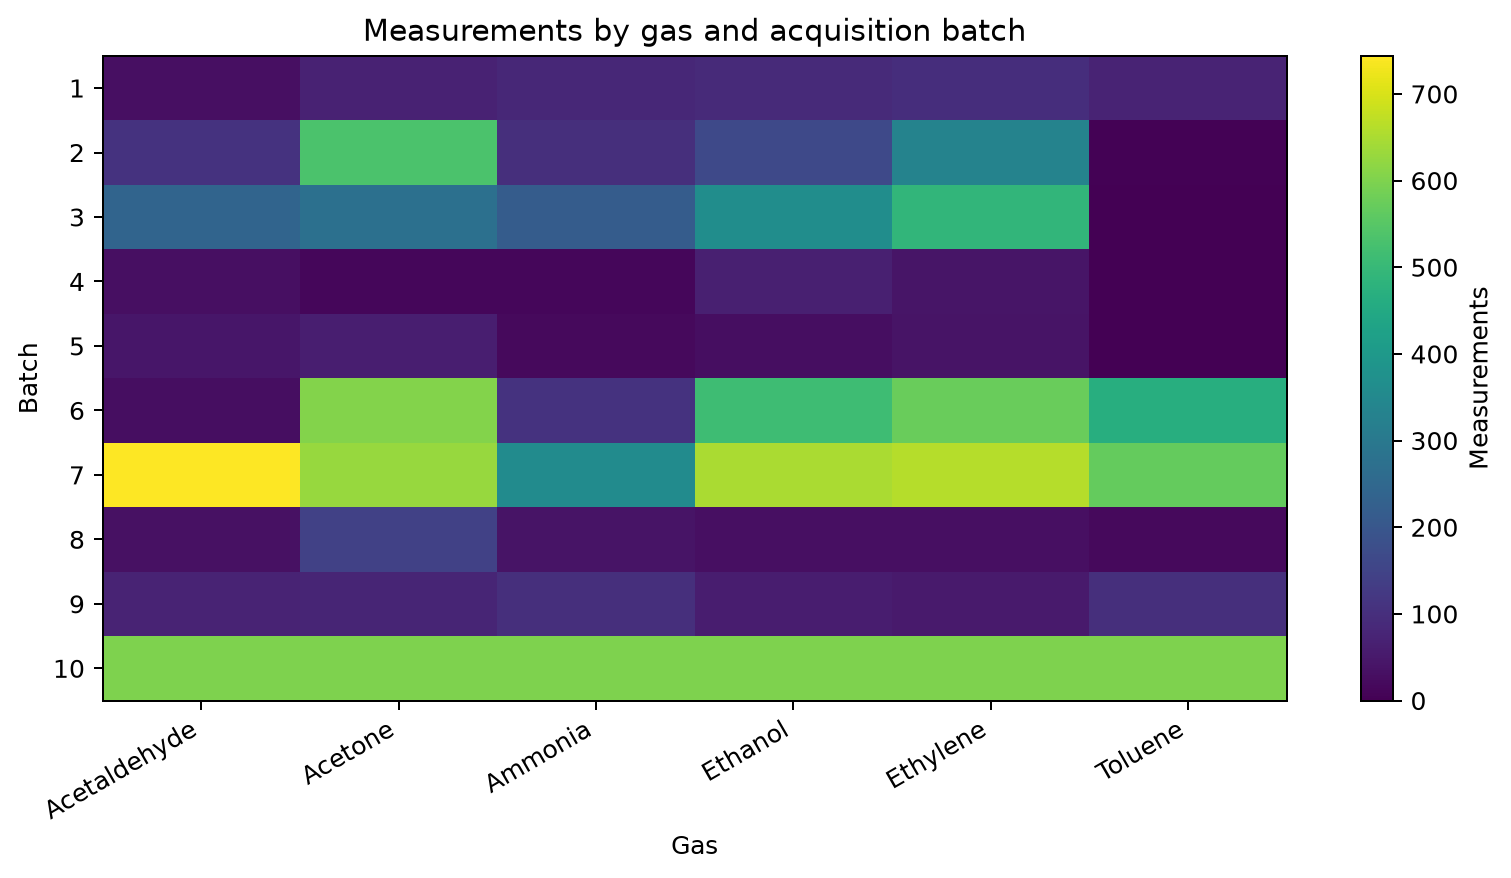
\includegraphics[width=\linewidth]{02_batch_gas_heatmap.png}
\caption{Measurements by gas and acquisition batch. The later-batch protocol uses batches 1--5 for training and batches 6--10 for testing, so the batch distribution is part of the experimental difficulty rather than a nuisance to remove.}
\label{fig:batch_heatmap}
\end{figure}

\section{Methodology}
\label{sec:methods}
\subsection{Reproducible Pipeline}
The benchmark is implemented as independent Python modules and scripts. Data acquisition records the official URL, archive hash, and per-batch hashes. Protocol construction writes the split summary and leakage audit before model training. A single fixed random seed (42) governs the random hold-out split, cross-validation folds, randomized hyperparameter search, bootstrap resampling, and clustering initialization, and is recorded together with package versions and profile parameters in the generated experiment manifest. The implementation uses scikit-learn for most estimators and utilities \cite{pedregosa2011}, XGBoost for gradient-boosted trees \cite{chen2016}, and joblib serialization for trained artifacts.

\subsection{Supervised Models}
For classification, the benchmark evaluates a prior-probability dummy classifier, Random Forest \cite{breiman2001}, XGBoost \cite{chen2016}, support vector classification following the SVM family implemented in LIBSVM-like tooling \cite{chang2011}, and a multilayer perceptron trained by back-propagation \cite{rumelhart1986}. Regression uses the analogous dummy median regressor, Random Forest regressor, XGBoost regressor, support vector regressor, and MLP regressor.

SVM, SVR, and MLP are wrapped in \texttt{Pipeline(StandardScaler, model)}. This is important because scaling is fit inside cross-validation folds rather than globally before tuning. Randomized hyperparameter search is performed only on the training partition of the active protocol. The temporal protocol uses \texttt{GroupKFold} over training batches only; batches 6--10 never participate in tuning.

\subsection{Metrics and Selection}
Classification reports accuracy, balanced accuracy, macro precision, macro recall, macro-F1, weighted-F1, and Matthews correlation coefficient (MCC). Regression reports mean absolute error (MAE), root mean squared error (RMSE), median absolute error, and $R^2$. The main tables in Section~\ref{sec:results} report a compact subset of these metrics; the remaining metrics are reported in the auxiliary tables described in Section~\ref{sec:results}. Candidate models for each protocol are selected from training cross-validation scores (macro-F1 for classification, negative RMSE for regression) rather than from held-out test performance, so test-set results never influence model selection.

Uncertainty is quantified with a non-parametric, record-level percentile bootstrap over the held-out predictions of each protocol: the test-set predictions are resampled with replacement for 1,000 iterations (FULL profile), and the 2.5th and 97.5th percentiles of the resulting metric distribution are reported as a 95\% confidence interval. The record-level bootstrap intervals indicate that the observed differences are stable under resampling of predictions within the fixed held-out set of each protocol; they do not refit the model and do not quantify uncertainty across alternative acquisition batches, alternative temporal partitions, or repeated data collection.

Training time is measured as wall-clock fitting time for the refitted best estimator on the full training partition. Inference time is measured by calling \texttt{predict} on the entire test partition 30 times (FULL profile) and reporting the median total wall-clock time, divided by the number of test observations to obtain a per-sample estimate in microseconds; this is a batch-normalized average rather than a per-observation measurement, since predictions are issued for the full test array in a single call. All measurements were collected on a single workstation (Intel Core i7-14700K, 20 cores/28 threads, Windows 11 Pro) with no other computationally intensive process running concurrently, using the Python and package versions recorded in the generated experiment manifest; no GPU acceleration was used. Timing values are hardware-dependent and are reported for relative comparison across models within this run rather than as absolute deployment figures.

\subsection{Feature Importance}
Permutation importance is computed on a bounded sample from the temporal test set for the models selected by temporal training cross-validation. The purpose is descriptive: permutation importance estimates the predictive sensitivity of a fitted model to each feature under permutation and does not establish causal relevance. For classification, the scoring function is macro-F1, so importance is reported as the mean decrease in macro-F1 after permutation. For regression, the scoring function is negative RMSE; because scikit-learn computes importance as the baseline score minus the permuted score, and both scores are negative RMSE values, the raw output already equals the increase in RMSE (ppmv) caused by permutation. To avoid the confusing double-negative phrasing of the raw scikit-learn scoring convention, this quantity is reported and labeled directly as the increase in RMSE (ppmv) after permutation, with no sign transformation applied.

\subsection{Unsupervised Analysis}
For clustering, a bounded sample of observations (5,000 in the QUICK profile, 10,000 in the FULL profile) is standardized and reduced by principal component analysis (PCA) to retain at least 95\% explained variance. k-Means is evaluated for $k=2,\ldots,10$ following the classical partitioning approach \cite{macqueen1967}; silhouette \cite{rousseeuw1987}, Davies-Bouldin \cite{davies1979}, and Calinski-Harabasz \cite{calinski1974} scores are computed for every $k$ as an unsupervised sensitivity analysis. The primary k-Means row reported in Table~\ref{tab:clustering} uses $k=6$, fixed to match the known number of gas classes; this configuration is therefore a reference partition aligned with the label cardinality rather than a value chosen by an internal validity criterion. The full sensitivity curve, including which $k$ each internal criterion would select if used for unsupervised model selection, is shown in Fig.~\ref{fig:kmeans_sensitivity}.

DBSCAN \cite{ester1996} is evaluated over a grid of \texttt{min\_samples} $\in\{5,10,20\}$ and, for each \texttt{min\_samples}, four candidate values of \texttt{eps} taken from the $\{0.80,0.85,0.90,0.95\}$ quantiles of the \texttt{min\_samples}-th nearest-neighbor distance (Fig.~\ref{fig:dbscan_kdist}). Among the twelve resulting configurations, the one with the highest silhouette score (ties broken by the lowest noise fraction) among configurations with at least two non-noise clusters and at least 100 non-noise points is selected. Points labeled as noise (label $-1$) are excluded when computing silhouette, Davies-Bouldin, and Calinski-Harabasz, since these internal indices are not defined for a designated noise label; noise points are retained as a distinct label when computing ARI and NMI against gas and batch, since these external indices tolerate an additional label. Adjusted Rand index (ARI) and normalized mutual information (NMI) against gas and batch labels are reported only as post-hoc external diagnostics and are not used to select DBSCAN or k-Means parameters.

\section{Results}
\label{sec:results}
\subsection{Classification}
Table~\ref{tab:classification} reports classification performance under the FULL experimental profile; Table~\ref{tab:classification_secondary} reports the remaining Methods-declared metrics and serialized model size. Under the mixed-batch random split, XGBoost achieved the highest observed macro-F1 (0.996 [95\% CI: 0.993--0.998]), with Random Forest, MLP, and SVM within 0.002 macro-F1 of one another (0.994--0.995); the dummy baseline remained near 0.059. This mixed-batch performance is not treated as evidence of a leakage bug, since the direct leakage audit in Table~\ref{tab:data_protocol} confirms that features exclude targets and metadata and that random train/test indices are disjoint.

The later-batch protocol resulted in substantially lower performance for every non-dummy model. MLP obtained the highest observed temporal macro-F1 (0.571 [95\% CI: 0.565--0.578]), ahead of SVM (0.499), Random Forest (0.491), and XGBoost (0.474); this ranking differs from the mixed-batch ranking, in which XGBoost and Random Forest led and MLP and SVM trailed slightly, indicating that mixed-batch performance is not a reliable predictor of later-batch performance for this benchmark. Fig.~\ref{fig:classification_protocols} visualizes the protocol contrast, and Fig.~\ref{fig:classification_drift} shows the temporal-minus-random macro-F1 deltas. The largest degradation is observed for XGBoost ($\Delta=-0.522$) and Random Forest ($\Delta=-0.504$), while MLP shows the smallest degradation among the non-dummy models ($\Delta=-0.423$). This pattern is consistent with later-batch distribution shift, of which sensor drift is one candidate contributor alongside the smaller and less diverse later-batch training population (Section~\ref{sec:limitations}).

\begin{table*}[t]
\caption{Classification performance for the mixed-batch random and later-batch (temporal) protocols. Bracketed values are 95\% bootstrap confidence intervals over the held-out predictions.}
\label{tab:classification}
\centering
\scriptsize
\begin{tabular}{llrrllrr}
\toprule
Protocol & Model & Acc. & Bal. Acc. & Macro-F1 [95\% CI] & MCC [95\% CI] & Train (s) & Infer. ($\mu$s/sample) \\
\midrule
Random & XGBoost & 0.996 & 0.995 & 0.996 [0.993, 0.998] & 0.995 [0.992, 0.997] & 231.399 & 5.032 \\
Random & Random Forest & 0.995 & 0.995 & 0.995 [0.992, 0.998] & 0.994 [0.991, 0.997] & 40.464 & 43.608 \\
Random & MLP & 0.994 & 0.993 & 0.994 [0.991, 0.997] & 0.993 [0.990, 0.996] & 34.050 & 1.483 \\
Random & SVM & 0.994 & 0.993 & 0.994 [0.991, 0.997] & 0.993 [0.989, 0.996] & 127.043 & 72.814 \\
Random & Dummy & 0.216 & 0.167 & 0.059 [0.056, 0.063] & 0.000 [0.000, 0.000] & 0.001 & 0.031 \\
\midrule
Temporal & MLP & 0.631 & 0.616 & 0.571 [0.565, 0.578] & 0.580 [0.570, 0.590] & 8.439 & 1.223 \\
Temporal & SVM & 0.552 & 0.549 & 0.499 [0.492, 0.507] & 0.496 [0.486, 0.506] & 8.787 & 2.628 \\
Temporal & Random Forest & 0.542 & 0.530 & 0.491 [0.483, 0.499] & 0.465 [0.454, 0.475] & 13.336 & 7.235 \\
Temporal & XGBoost & 0.505 & 0.498 & 0.474 [0.466, 0.482] & 0.421 [0.409, 0.432] & 57.057 & 1.321 \\
Temporal & Dummy & 0.187 & 0.167 & 0.052 [0.051, 0.054] & 0.000 [0.000, 0.000] & 0.000 & 0.009 \\
\bottomrule
\end{tabular}
\end{table*}

\begin{table}[t]
\caption{Additional classification metrics (Section~\ref{sec:methods}) and serialized model size.}
\label{tab:classification_secondary}
\centering
\footnotesize
\begin{tabular}{llrrrr}
\toprule
Protocol & Model & M.Prec. & M.Rec. & W.-F1 & Size (MB) \\
\midrule
Random & XGBoost & 0.996 & 0.995 & 0.996 & 0.656 \\
Random & Random Forest & 0.996 & 0.995 & 0.995 & 3.021 \\
Random & MLP & 0.994 & 0.993 & 0.994 & 0.563 \\
Random & SVM & 0.994 & 0.993 & 0.994 & 1.336 \\
Random & Dummy & 0.036 & 0.167 & 0.077 & 0.001 \\
\midrule
Temporal & MLP & 0.563 & 0.616 & 0.582 & 0.199 \\
Temporal & SVM & 0.606 & 0.549 & 0.509 & 0.134 \\
Temporal & Random Forest & 0.478 & 0.530 & 0.508 & 0.725 \\
Temporal & XGBoost & 0.639 & 0.498 & 0.488 & 0.292 \\
Temporal & Dummy & 0.031 & 0.167 & 0.059 & 0.001 \\
\bottomrule
\end{tabular}
\end{table}

\begin{figure}[t]
\centering
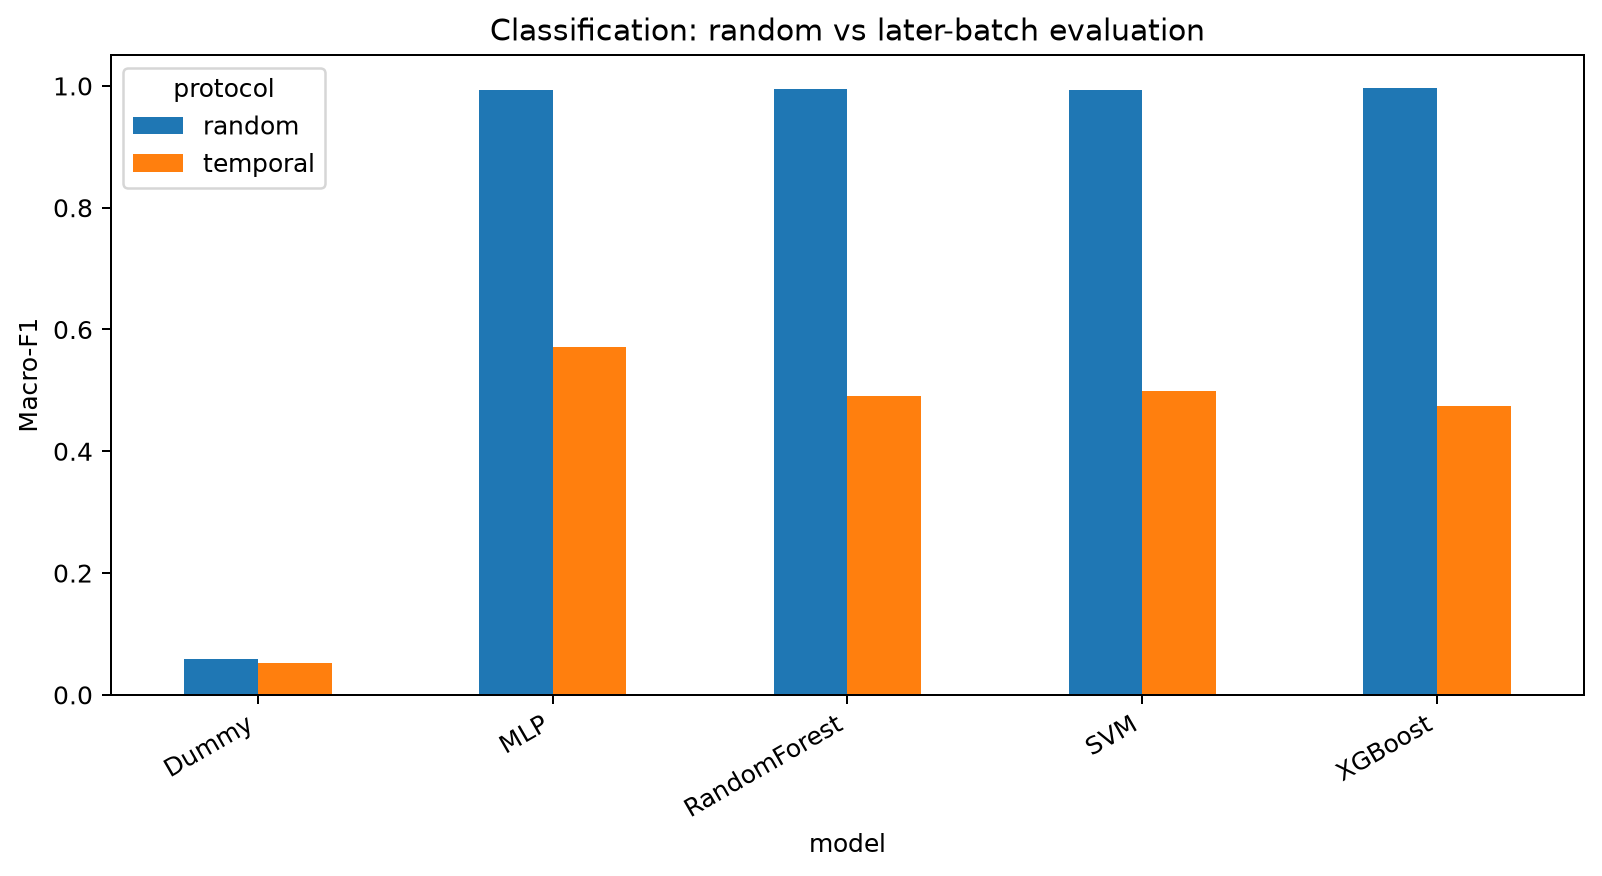
\includegraphics[width=\linewidth]{05_classification_random_vs_temporal.png}
\caption{Classification macro-F1 under the mixed-batch random and later-batch evaluation protocols. Every non-dummy model degrades under later-batch testing.}
\label{fig:classification_protocols}
\end{figure}

\begin{figure}[t]
\centering
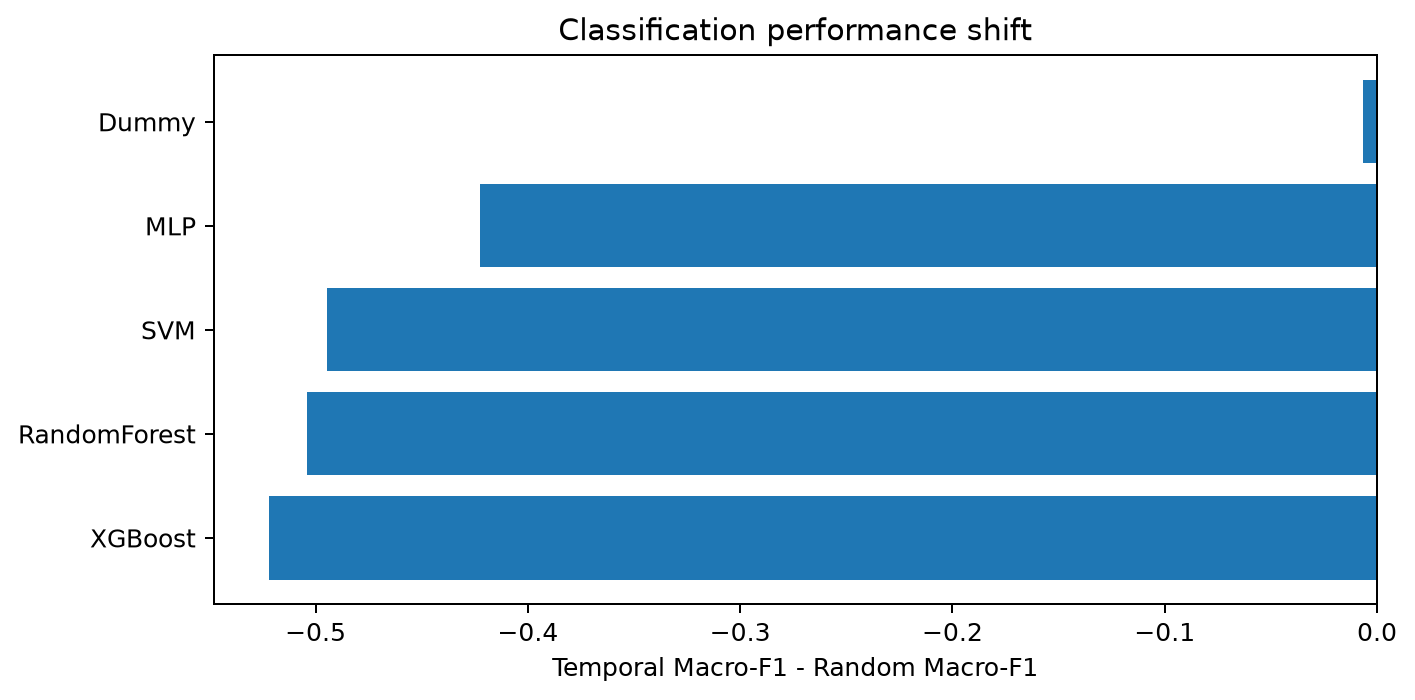
\includegraphics[width=\linewidth]{06_classification_drift_delta.png}
\caption{Temporal-minus-random macro-F1 deltas. Negative values indicate degradation when testing on later acquisition batches.}
\label{fig:classification_drift}
\end{figure}

The aggregate temporal macro-F1 of MLP (0.571) conceals substantial heterogeneity across gases (Table~\ref{tab:per_class}, Fig.~\ref{fig:confusion_temporal}). Acetone and Ethylene are recognized comparatively well (F1 of 0.895 and 0.875), Ammonia is intermediate (F1 0.816), and Ethanol shows high recall but low precision (0.959 and 0.433), indicating that many later-batch measurements of other gases are misclassified as Ethanol. Degradation is most severe for Acetaldehyde (F1 0.243) and, especially, Toluene, for which the temporal MLP achieves an F1 of only 0.002: Toluene is almost entirely absorbed into other predicted classes under later-batch testing. This class-concentrated failure pattern would not be visible from the aggregate macro-F1 alone and indicates that later-batch degradation is not uniform across gases.

\begin{table}[t]
\caption{Per-class diagnostics for the later-batch protocol, MLP classifier (selected by temporal training cross-validation).}
\label{tab:per_class}
\centering
\footnotesize
\begin{tabular}{lrrrr}
\toprule
Gas & Precision & Recall & F1 & Support \\
\midrule
Ethanol & 0.433 & 0.959 & 0.596 & 1854 \\
Ethylene & 0.900 & 0.851 & 0.875 & 1921 \\
Ammonia & 0.816 & 0.817 & 0.816 & 1210 \\
Acetaldehyde & 0.285 & 0.211 & 0.243 & 1481 \\
Acetone & 0.934 & 0.860 & 0.895 & 2057 \\
Toluene & 0.014 & 0.001 & 0.002 & 1754 \\
\bottomrule
\end{tabular}
\end{table}

\begin{figure}[t]
\centering
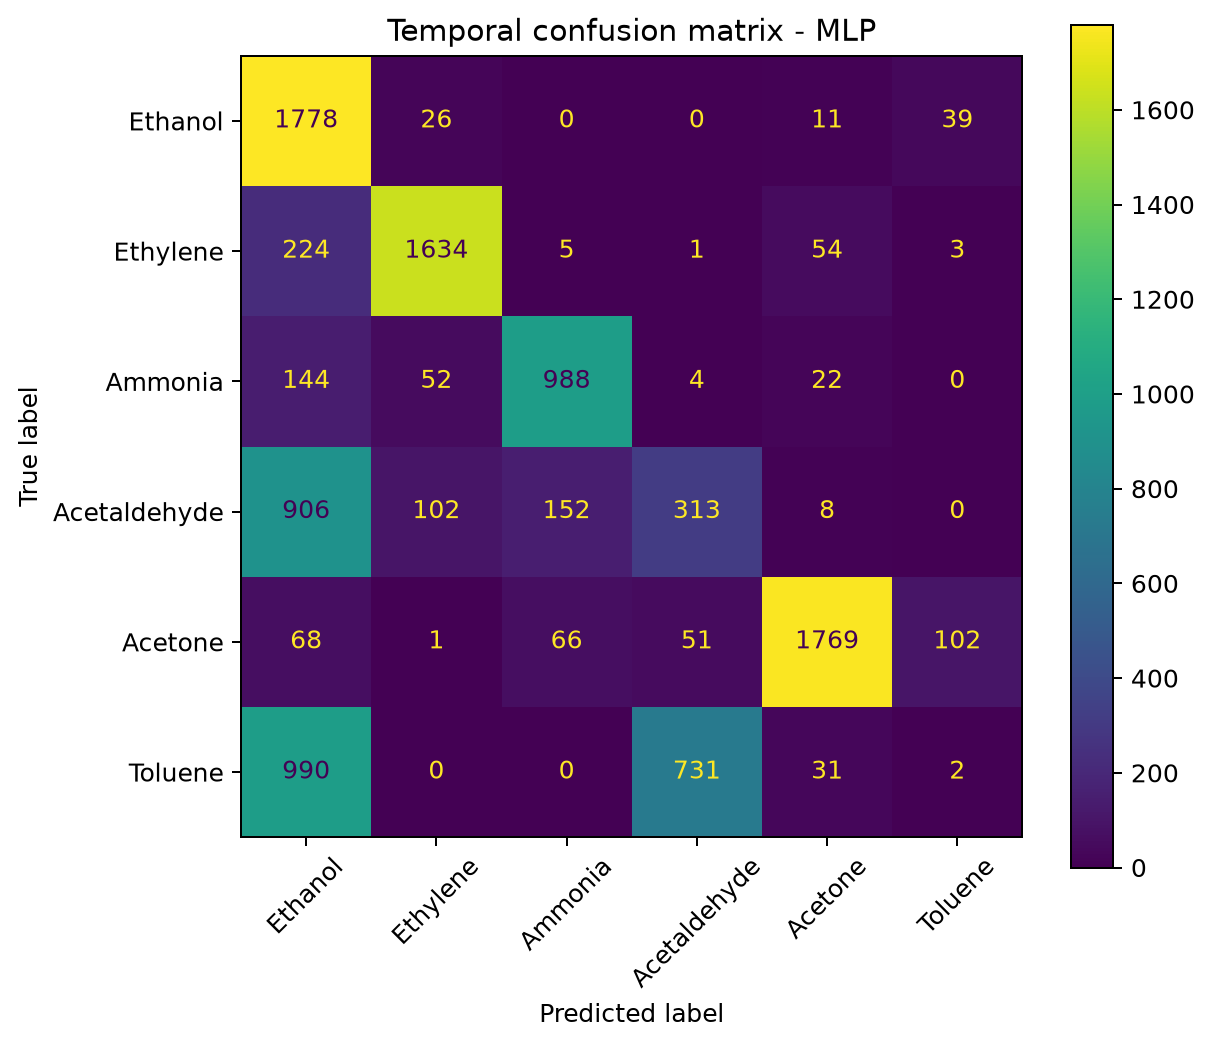
\includegraphics[width=\linewidth]{07_confusion_temporal_mlp.png}
\caption{Later-batch confusion matrix for the MLP classifier, the model selected by temporal training cross-validation. Rows are true gas labels and columns are predicted labels; counts are raw test-set counts (Table~\ref{tab:per_class} reports the corresponding precision, recall, and F1 per class).}
\label{fig:confusion_temporal}
\end{figure}

\subsection{Regression}
Table~\ref{tab:regression} reports concentration-estimation results under the FULL experimental profile. In the mixed-batch random protocol, Random Forest obtained the lowest observed RMSE (30.098 ppmv [95\% CI: 20.676--41.254]), with XGBoost (31.846 ppmv) and MLP (31.394 ppmv) close behind and SVR somewhat higher (35.959 ppmv); all four learned regressors improved sharply over the dummy median baseline (189.886 ppmv).

Errors increased for every learned regressor under the later-batch protocol. SVR obtained the lowest observed temporal RMSE (113.575 ppmv [95\% CI: 108.581--118.608]), ahead of XGBoost (118.614 ppmv), Random Forest (132.562 ppmv), and MLP (134.010 ppmv); as with classification, the temporal ranking differs from the mixed-batch ranking, where SVR was the weakest learned regressor. Fig.~\ref{fig:regression_protocols} compares mixed-batch and later-batch RMSE, and Fig.~\ref{fig:regression_drift} presents the temporal-minus-random error changes. RMSE increased by 77.6--102.6 ppmv for the learned regressors ($\Delta_{\text{Random Forest}}=+102.5$, $\Delta_{\text{MLP}}=+102.6$, $\Delta_{\text{XGBoost}}=+86.8$, $\Delta_{\text{SVR}}=+77.6$), while the dummy baseline changed only marginally between protocols. This mirrors the classification result: mixed-batch accuracy does not transfer directly to later-batch performance, and the model with the strongest mixed-batch score is not necessarily the model with the strongest later-batch score.

\begin{table*}[t]
\caption{Regression performance for concentration estimation under the mixed-batch random and later-batch (temporal) protocols. Bracketed values are 95\% bootstrap confidence intervals over the held-out predictions.}
\label{tab:regression}
\centering
\scriptsize
\begin{tabular}{llrrllrrr}
\toprule
Protocol & Model & MAE [95\% CI] & Median AE & RMSE [95\% CI] & $R^2$ & Train (s) & Infer. ($\mu$s/sample) & Size (MB) \\
\midrule
Random & Random Forest & 8.469 [7.407, 9.681] & 2.225 & 30.098 [20.676, 41.254] & 0.972 & 103.650 & 19.367 & 9.070 \\
Random & XGBoost & 10.328 [9.269, 11.555] & 3.896 & 31.846 [22.697, 42.750] & 0.969 & 49.989 & 2.764 & 0.393 \\
Random & MLP & 11.090 [10.058, 12.210] & 4.655 & 31.394 [23.237, 40.503] & 0.970 & 251.391 & 2.332 & 0.560 \\
Random & SVR & 12.799 [11.549, 14.110] & 4.657 & 35.959 [27.694, 45.916] & 0.960 & 143.050 & 542.865 & 8.902 \\
Random & Dummy & 108.093 [102.772, 113.764] & 70.000 & 189.886 [178.007, 202.264] & -0.113 & 0.001 & 0.007 & 0.001 \\
\midrule
Temporal & SVR & 55.872 [53.890, 57.754] & 28.155 & 113.575 [108.581, 118.608] & 0.631 & 6.816 & 140.205 & 2.663 \\
Temporal & XGBoost & 64.274 [62.328, 66.239] & 35.473 & 118.614 [113.696, 123.131] & 0.597 & 23.214 & 0.843 & 0.122 \\
Temporal & Random Forest & 63.997 [61.667, 66.137] & 31.642 & 132.562 [126.738, 137.807] & 0.497 & 20.628 & 6.953 & 4.018 \\
Temporal & MLP & 82.016 [79.912, 84.157] & 54.458 & 134.010 [129.233, 138.828] & 0.486 & 77.863 & 1.441 & 0.194 \\
Temporal & Dummy & 116.975 [114.220, 119.834] & 100.000 & 186.882 [180.679, 192.901] & -0.000 & 0.001 & 0.001 & 0.001 \\
\bottomrule
\end{tabular}
\end{table*}

\begin{figure}[t]
\centering
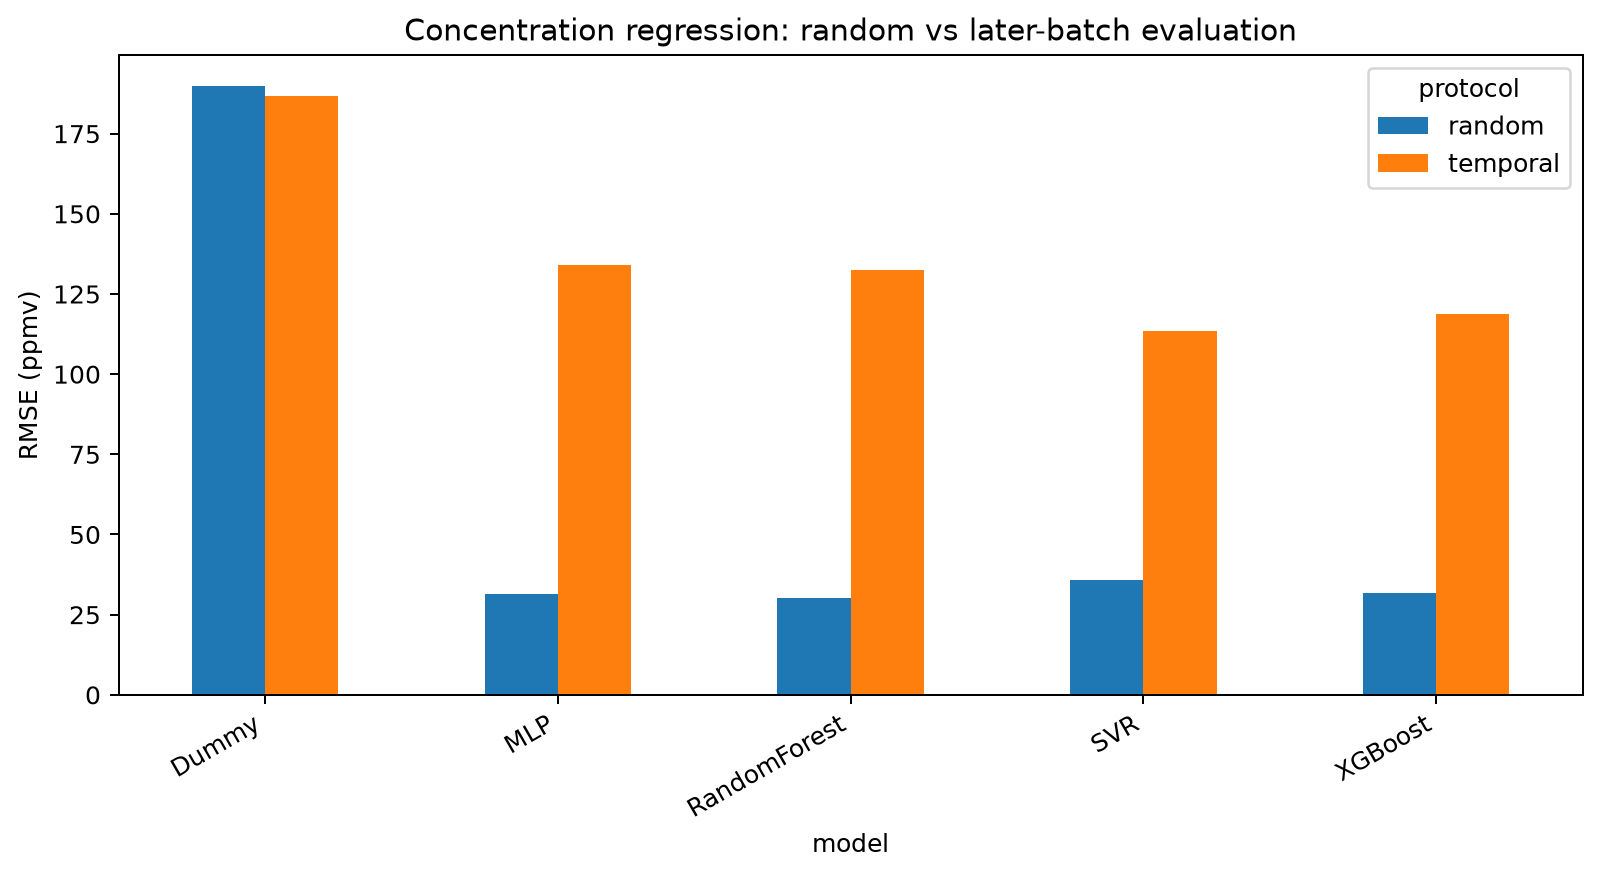
\includegraphics[width=\linewidth]{08_regression_random_vs_temporal.png}
\caption{Regression RMSE under the mixed-batch random and later-batch evaluation protocols. Learned models are accurate in the random split but experience large RMSE increases under later-batch testing.}
\label{fig:regression_protocols}
\end{figure}

\begin{figure}[t]
\centering
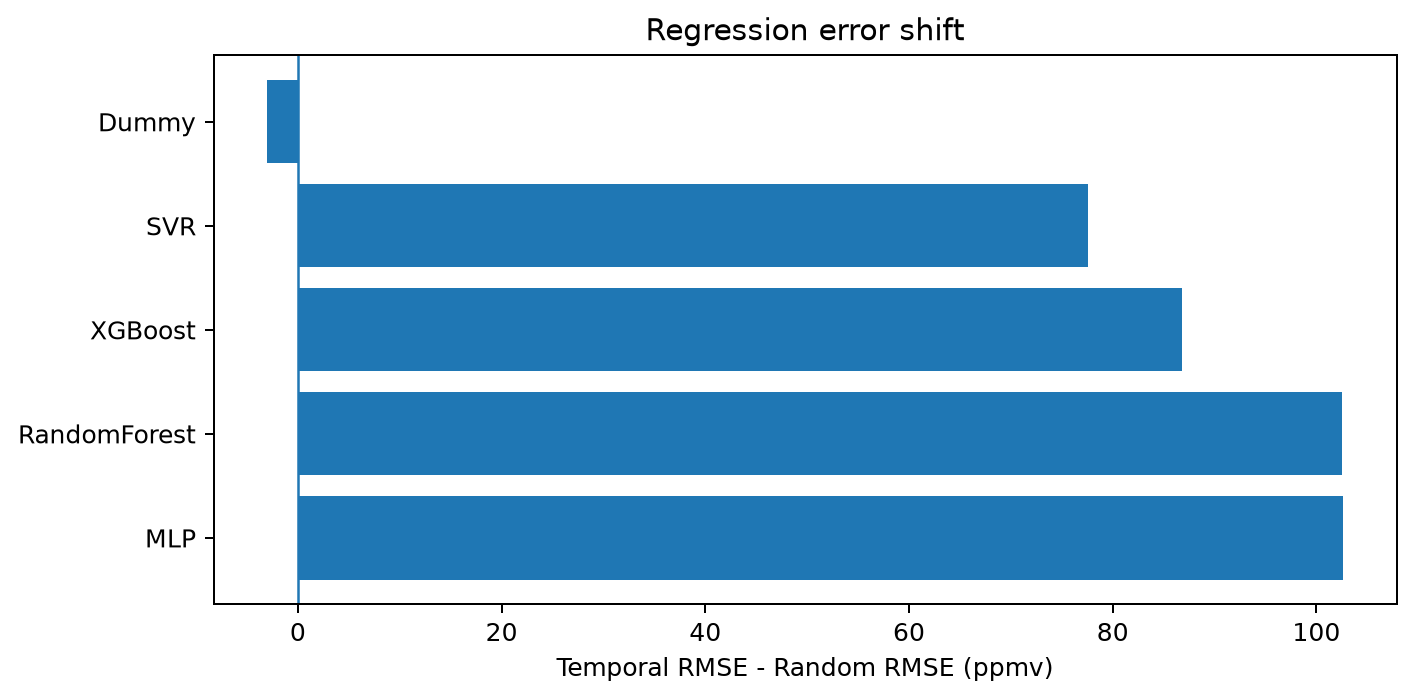
\includegraphics[width=\linewidth]{09_regression_drift_delta.png}
\caption{Temporal-minus-random RMSE deltas. Positive values indicate increased concentration-estimation error on later batches.}
\label{fig:regression_drift}
\end{figure}

Because concentration ranges differ substantially across gases, the global temporal RMSE and MAE reported in Table~\ref{tab:regression} can obscure heterogeneous per-gas behavior. Table~\ref{tab:per_gas} breaks down the later-batch error of SVR, the best temporal regressor by training cross-validation, by gas. Ethanol and Ethylene, whose concentrations in this dataset do not exceed 250--300~ppmv, show the lowest absolute error (RMSE 37.6 and 41.7~ppmv). Acetone and Ammonia, whose concentrations extend to 1{,}000~ppmv, show much larger absolute error (RMSE 203.1 and 161.0~ppmv); part of this gap is consistent with their wider concentration range rather than a qualitatively different estimation difficulty. Toluene and Acetaldehyde fall in between. This heterogeneity indicates that the global RMSE in Table~\ref{tab:regression} is driven disproportionately by the high-concentration-range gases.

\begin{table}[t]
\caption{Per-gas later-batch regression error, SVR regressor (selected by temporal training cross-validation).}
\label{tab:per_gas}
\centering
\footnotesize
\begin{tabular}{lrrrr}
\toprule
Gas & $N$ & MAE (ppmv) & RMSE (ppmv) & Range (ppmv) \\
\midrule
Ethanol & 1854 & 31.447 & 37.609 & 2.5--250 \\
Ethylene & 1921 & 29.814 & 41.691 & 2.5--300 \\
Acetaldehyde & 1481 & 39.123 & 61.494 & 2.5--300 \\
Toluene & 1754 & 43.582 & 52.196 & 1.0--230 \\
Ammonia & 1210 & 96.992 & 161.041 & 2.5--1000 \\
Acetone & 2057 & 100.574 & 203.094 & 10.0--1000 \\
\bottomrule
\end{tabular}
\end{table}

\subsection{Permutation Importance}
The temporal training-CV procedure selected MLP for classification importance and SVR for regression importance, consistent with the models selected in the classification and regression subsections above. Fig.~\ref{fig:importance} shows the top temporal permutation importances. For classification, the most influential features are \texttt{feature\_105}, \texttt{feature\_097}, and \texttt{feature\_025}; permuting \texttt{feature\_105} decreases macro-F1 by 0.0274 on average. For regression, the most influential features are \texttt{feature\_106}, \texttt{feature\_098}, and \texttt{feature\_110}; permuting \texttt{feature\_106} increases RMSE by 10.50~ppmv on average. The two importance rankings only partially overlap (\texttt{feature\_097}, \texttt{feature\_098}, \texttt{feature\_105}, and \texttt{feature\_110} appear among the top features for both tasks), which is expected given that classification and regression are trained as independent tasks on different targets. These values are model-specific predictive sensitivities and should not be interpreted as causal or feature-intrinsic importance.

\begin{figure*}[t]
\centering
\begin{minipage}{0.48\textwidth}
\centering
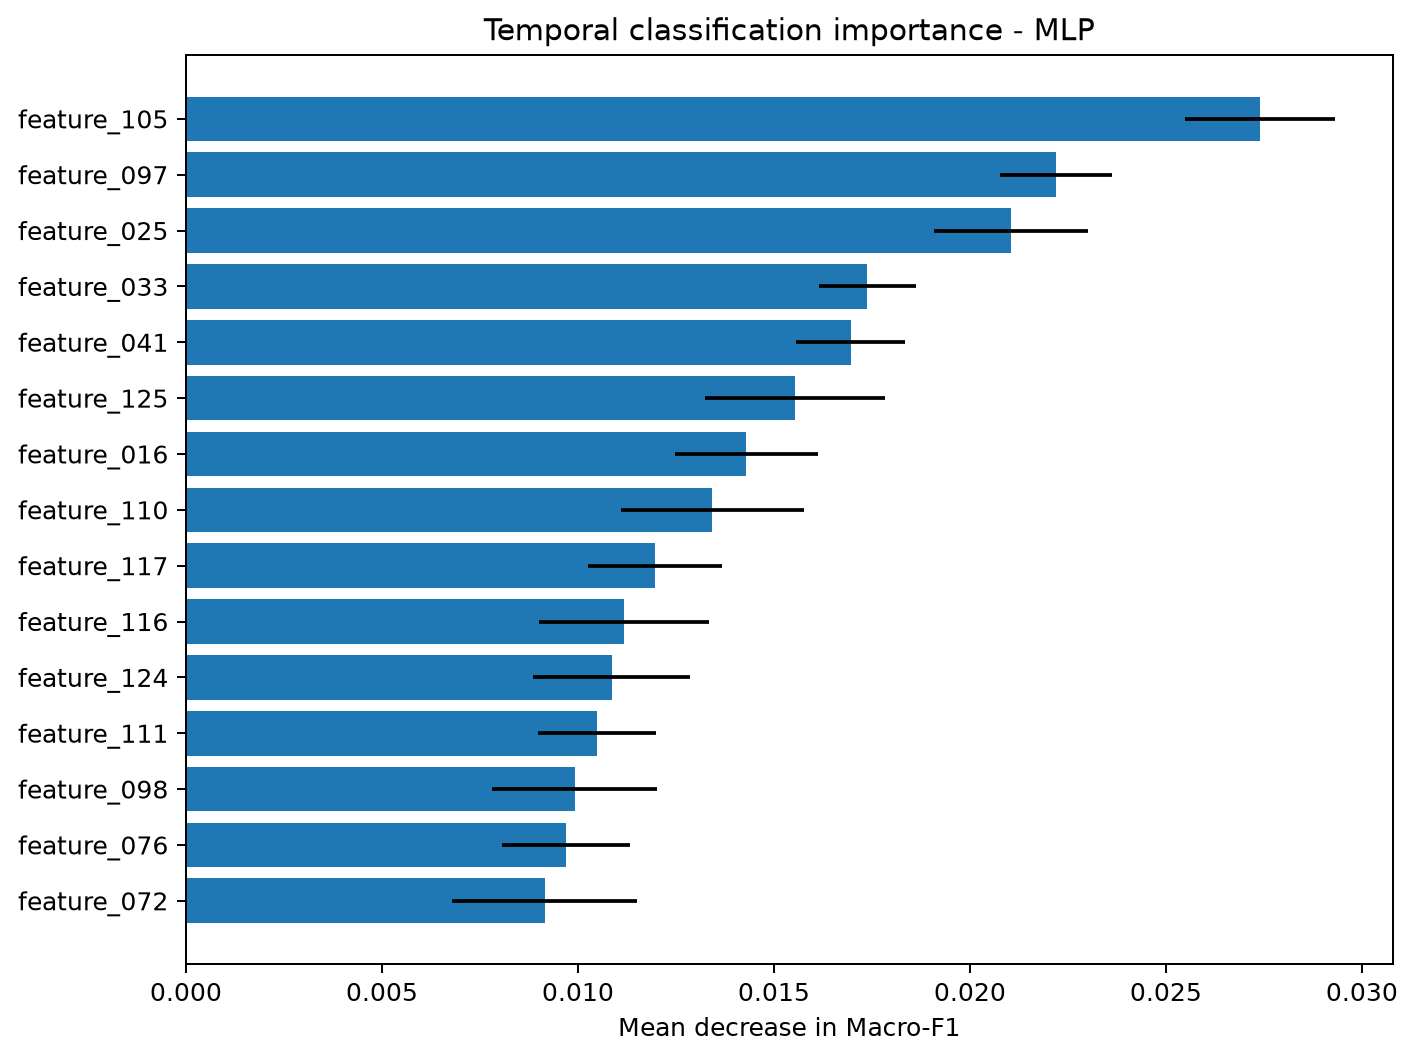
\includegraphics[width=\linewidth]{10_classification_permutation_importance.png}
\end{minipage}
\hfill
\begin{minipage}{0.48\textwidth}
\centering
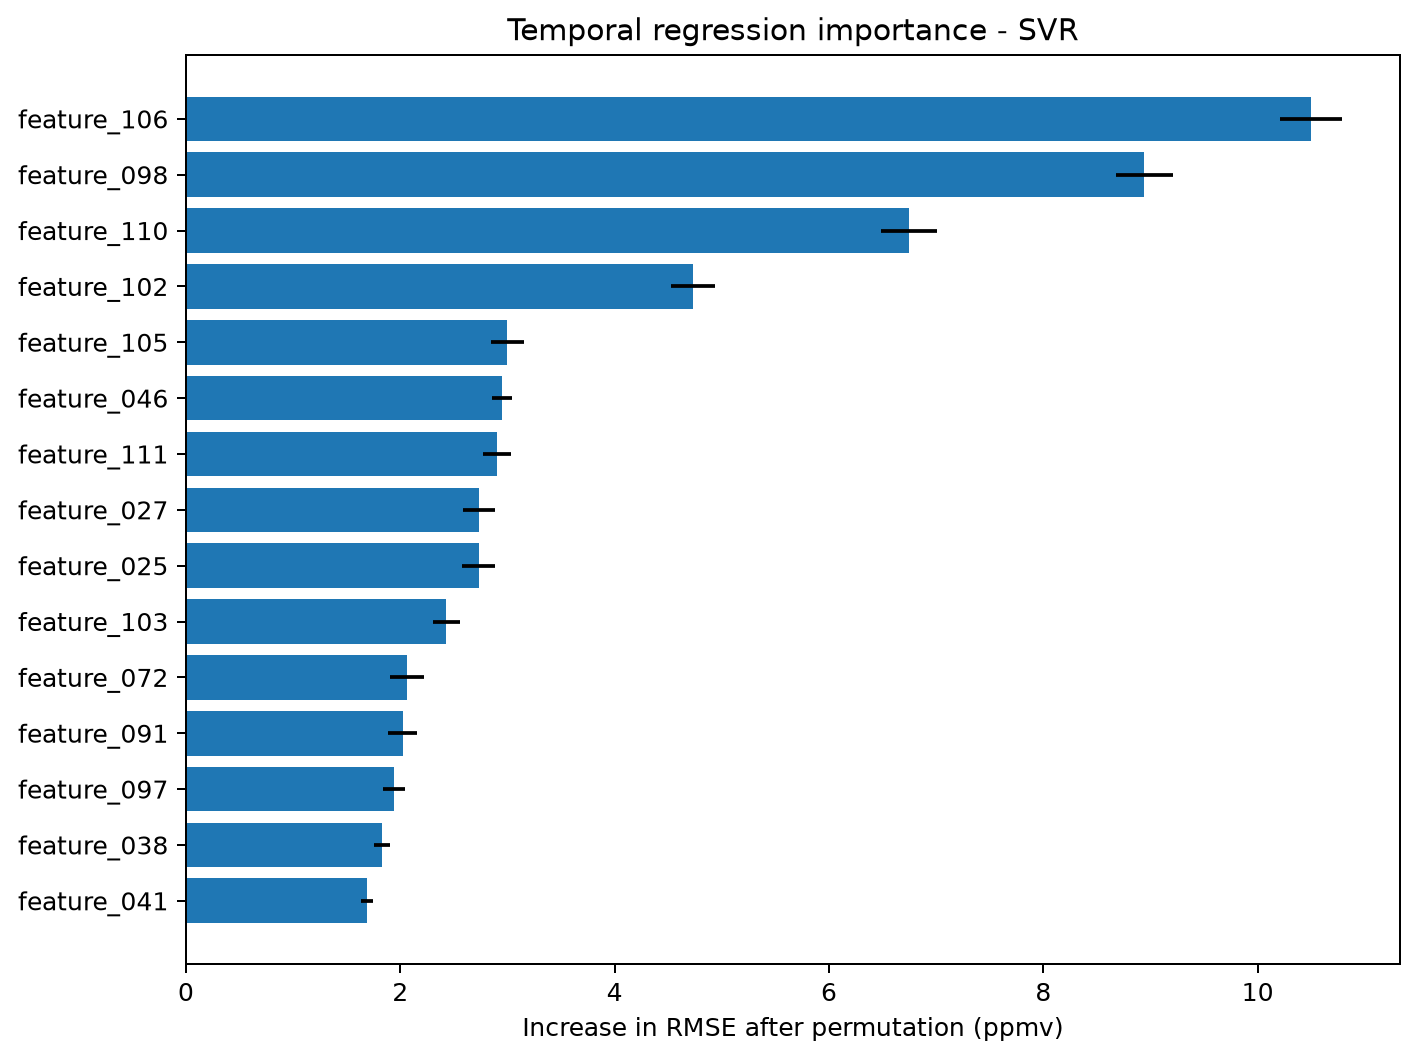
\includegraphics[width=\linewidth]{11_regression_permutation_importance.png}
\end{minipage}
\caption{Permutation importance for the later-batch classification and regression models selected by training cross-validation. Importance is predictive and model-dependent, not causal; the regression panel reports the increase in RMSE (ppmv) after permutation.}
\label{fig:importance}
\end{figure*}

\subsection{Clustering}
\label{sec:results_clustering}
PCA retained 11 components to explain at least 95\% of variance in the FULL-profile clustering sample (10,000 observations). Table~\ref{tab:clustering} reports the reference k-Means partition and the selected DBSCAN configuration against both external labels, as required to address RQ4. The reference k-Means partition ($k=6$, fixed to the number of gas classes) obtains silhouette 0.343 and weak external alignment with gas identity (ARI 0.090; NMI 0.242) and even weaker alignment with acquisition batch (ARI 0.045; NMI 0.106). Fig.~\ref{fig:kmeans_sensitivity} shows that no internal criterion in the $k=2,\ldots,10$ sensitivity sweep selects $k=6$: silhouette and Calinski-Harabasz both favor $k=2$, and Davies-Bouldin favors $k=3$, all with modest gas alignment (ARI $\leq 0.09$ throughout the sweep). This confirms that the $k=6$ partition is best read as a reference partition aligned with the known label cardinality rather than an unsupervised discovery of six chemically meaningful clusters.

The selected DBSCAN configuration (\texttt{eps=4.4662}, \texttt{min\_samples=20}) was chosen by the highest-silhouette criterion among the twelve searched grid configurations; Fig.~\ref{fig:dbscan_kdist} shows the $k$-distance diagnostic from which the four candidate eps quantiles were derived for this \texttt{min\_samples}. This configuration finds 4 clusters with 3.7\% noise and a higher silhouette than k-Means (0.498), but its ARI/NMI against both gas and batch are near zero (gas: ARI $-0.004$, NMI 0.029; batch: ARI 0.004, NMI 0.045). Internal cluster validity and external label alignment therefore diverge for DBSCAN: the partition is comparatively well separated in the PCA space but does not correspond to either gas identity or acquisition batch. Fig.~\ref{fig:clustering_labels} illustrates the PCA projections colored by gas identity and by acquisition batch, and Fig.~\ref{fig:clustering_algorithms} shows the corresponding k-Means and selected DBSCAN partitions of the same PCA space.

\begin{table*}[t]
\caption{Clustering summary on the FULL-profile sample (10,000 observations): reference k-Means partition ($k=6$) and selected DBSCAN configuration, against both gas and acquisition-batch external labels.}
\label{tab:clustering}
\centering
\footnotesize
\begin{tabular}{lrrrrrrr}
\toprule
Method & Clust. & Noise (\%) & Sil. & ARI-gas & NMI-gas & ARI-batch & NMI-batch \\
\midrule
k-Means ($k=6$) & 6 & 0.0 & 0.343 & 0.090 & 0.242 & 0.045 & 0.106 \\
DBSCAN (\texttt{eps=4.4662,min\_samples=20}) & 4 & 3.7 & 0.498 & -0.004 & 0.029 & 0.004 & 0.045 \\
\bottomrule
\end{tabular}
\end{table*}

\begin{figure}[t]
\centering
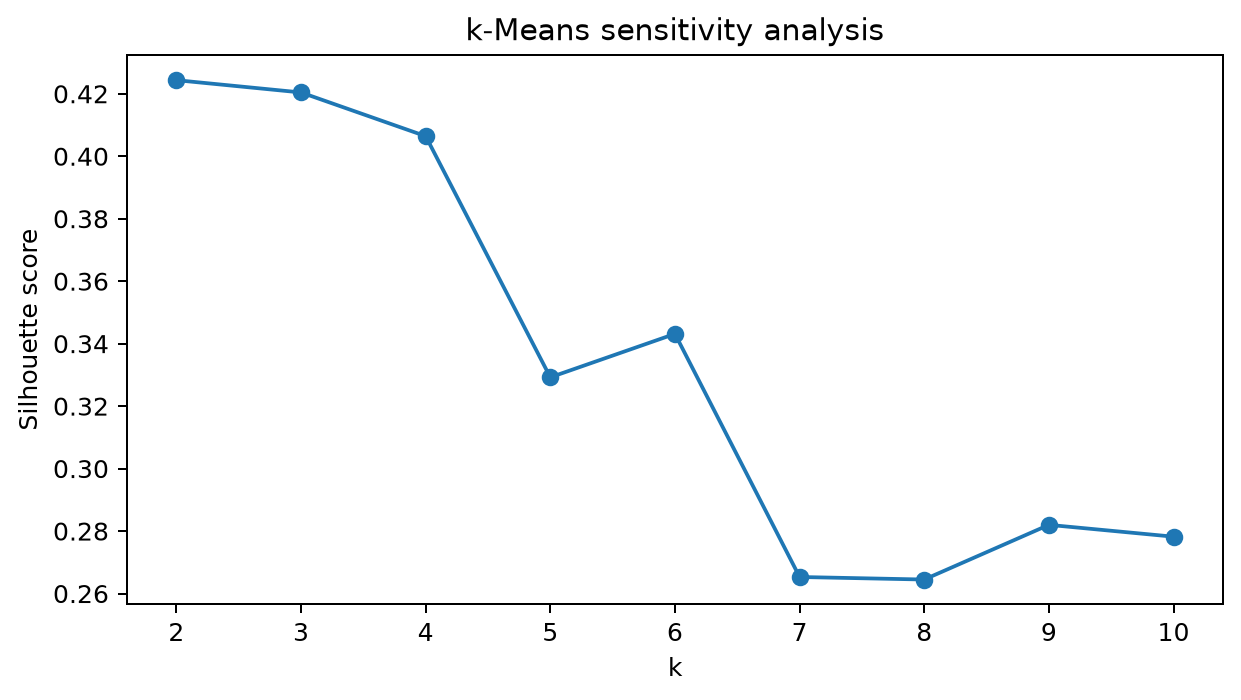
\includegraphics[width=\linewidth]{14_kmeans_sensitivity.png}
\caption{k-Means silhouette score as a function of the number of clusters $k$ on the FULL-profile clustering sample. The reference partition reported in Table~\ref{tab:clustering} fixes $k=6$ to match the number of gas classes rather than the silhouette-optimal $k$.}
\label{fig:kmeans_sensitivity}
\end{figure}

\begin{figure}[t]
\centering
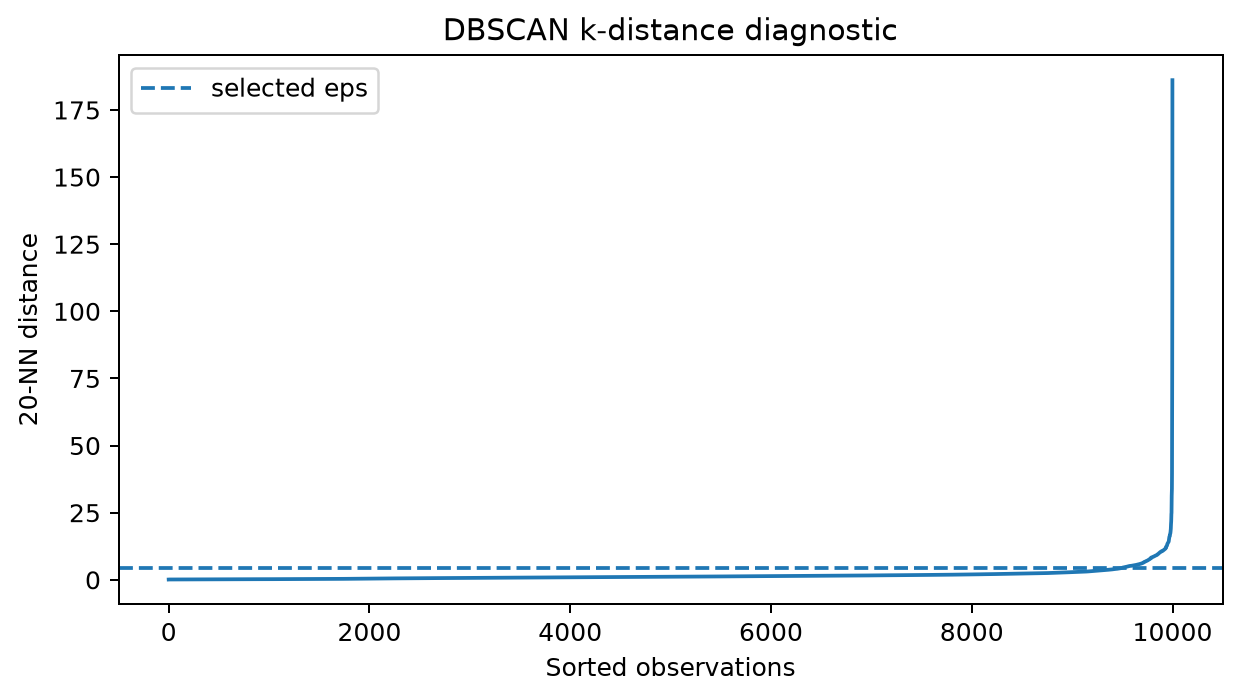
\includegraphics[width=\linewidth]{16_dbscan_k_distance.png}
\caption{$k$-distance diagnostic from which candidate eps quantiles were derived for \texttt{min\_samples=20} (Section~\ref{sec:methods}). The curve itself only supplies the four candidate eps values evaluated at this \texttt{min\_samples}; the dashed line marks the candidate ultimately selected from the full DBSCAN grid by the highest-silhouette criterion described in the text, not a value read directly off this diagnostic.}
\label{fig:dbscan_kdist}
\end{figure}

\begin{figure*}[t]
\centering
\begin{minipage}{0.48\textwidth}
\centering
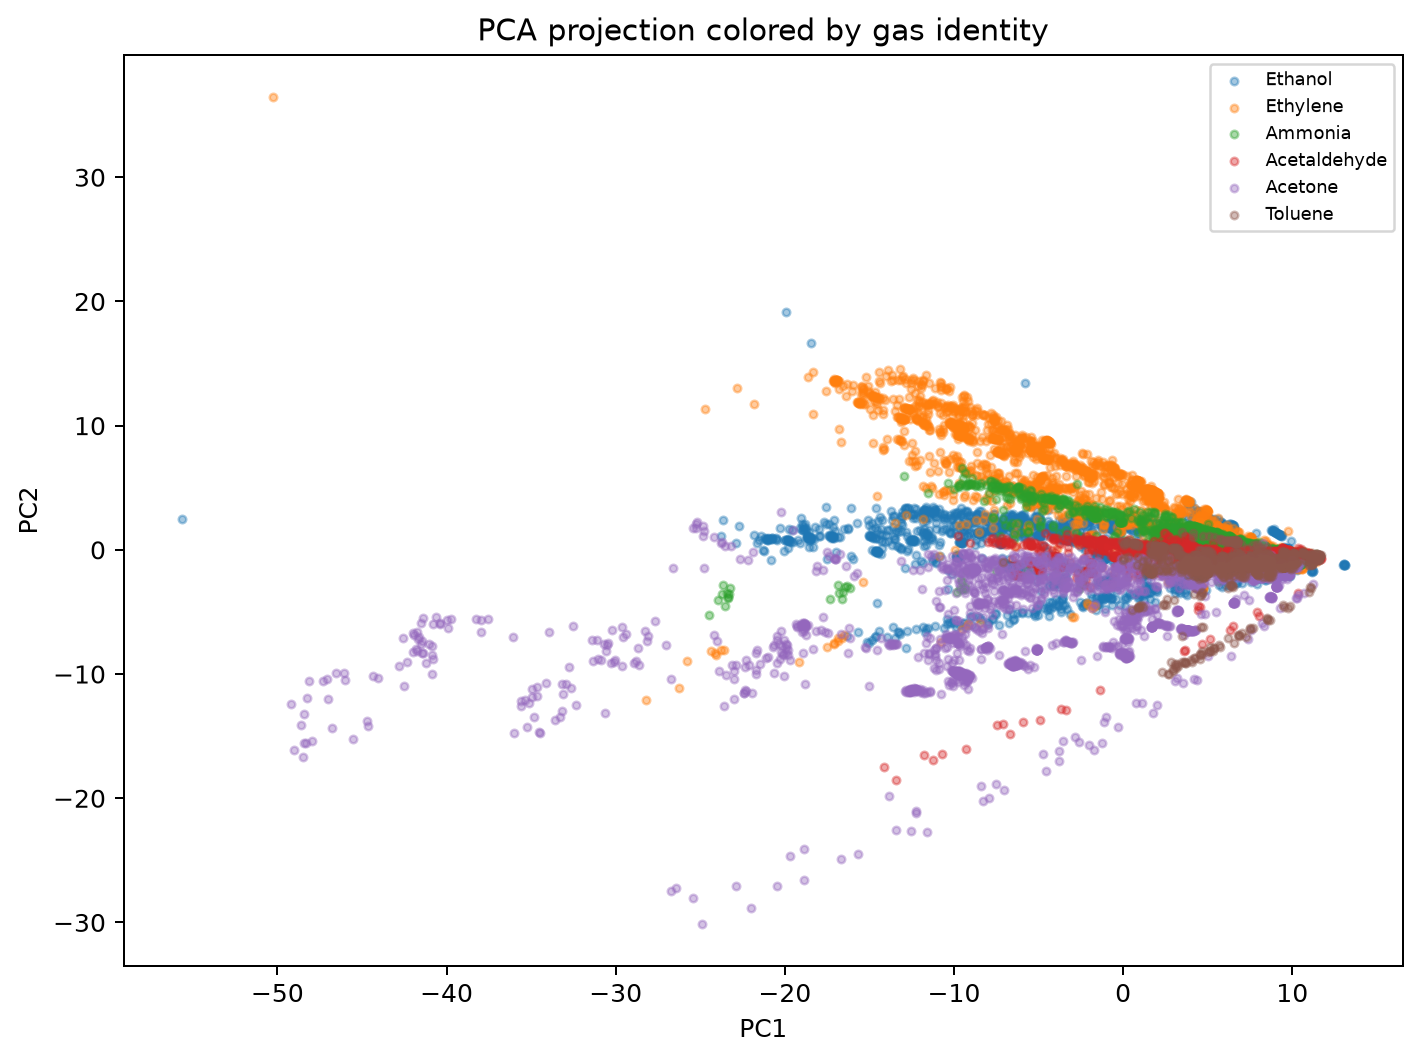
\includegraphics[width=\linewidth]{12_pca_by_gas.png}
\end{minipage}
\hfill
\begin{minipage}{0.48\textwidth}
\centering
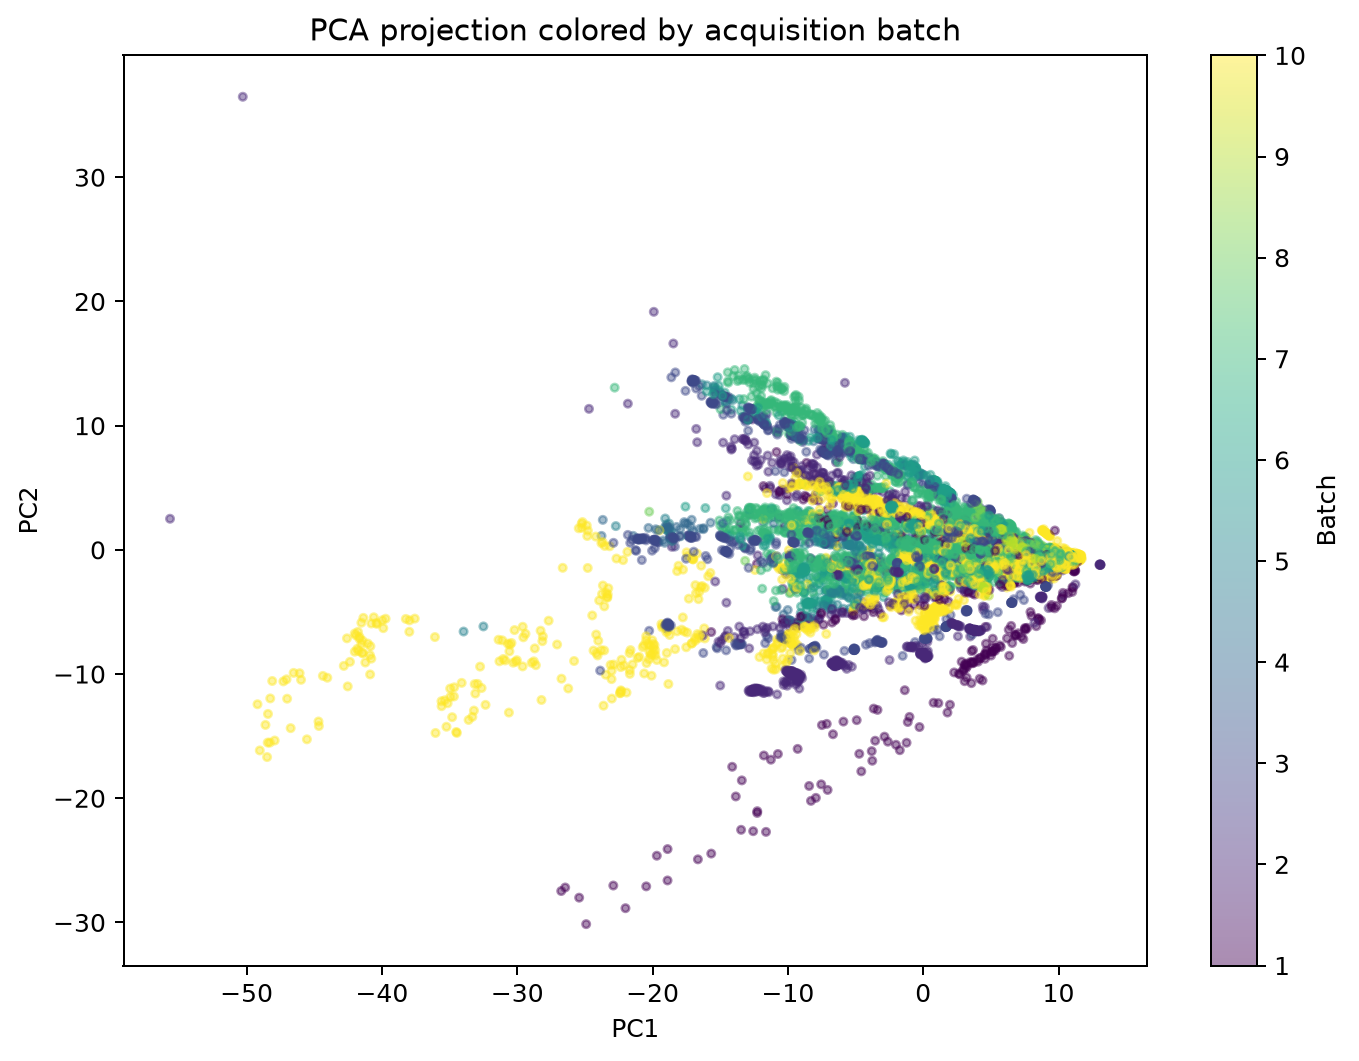
\includegraphics[width=\linewidth]{13_pca_by_batch_clustering_sample.png}
\end{minipage}
\caption{PCA projection of the clustering sample colored by gas identity (left) and by acquisition batch (right). These plots are exploratory and complement the quantitative external-alignment summary in Table~\ref{tab:clustering}.}
\label{fig:clustering_labels}
\end{figure*}

\begin{figure*}[t]
\centering
\begin{minipage}{0.48\textwidth}
\centering
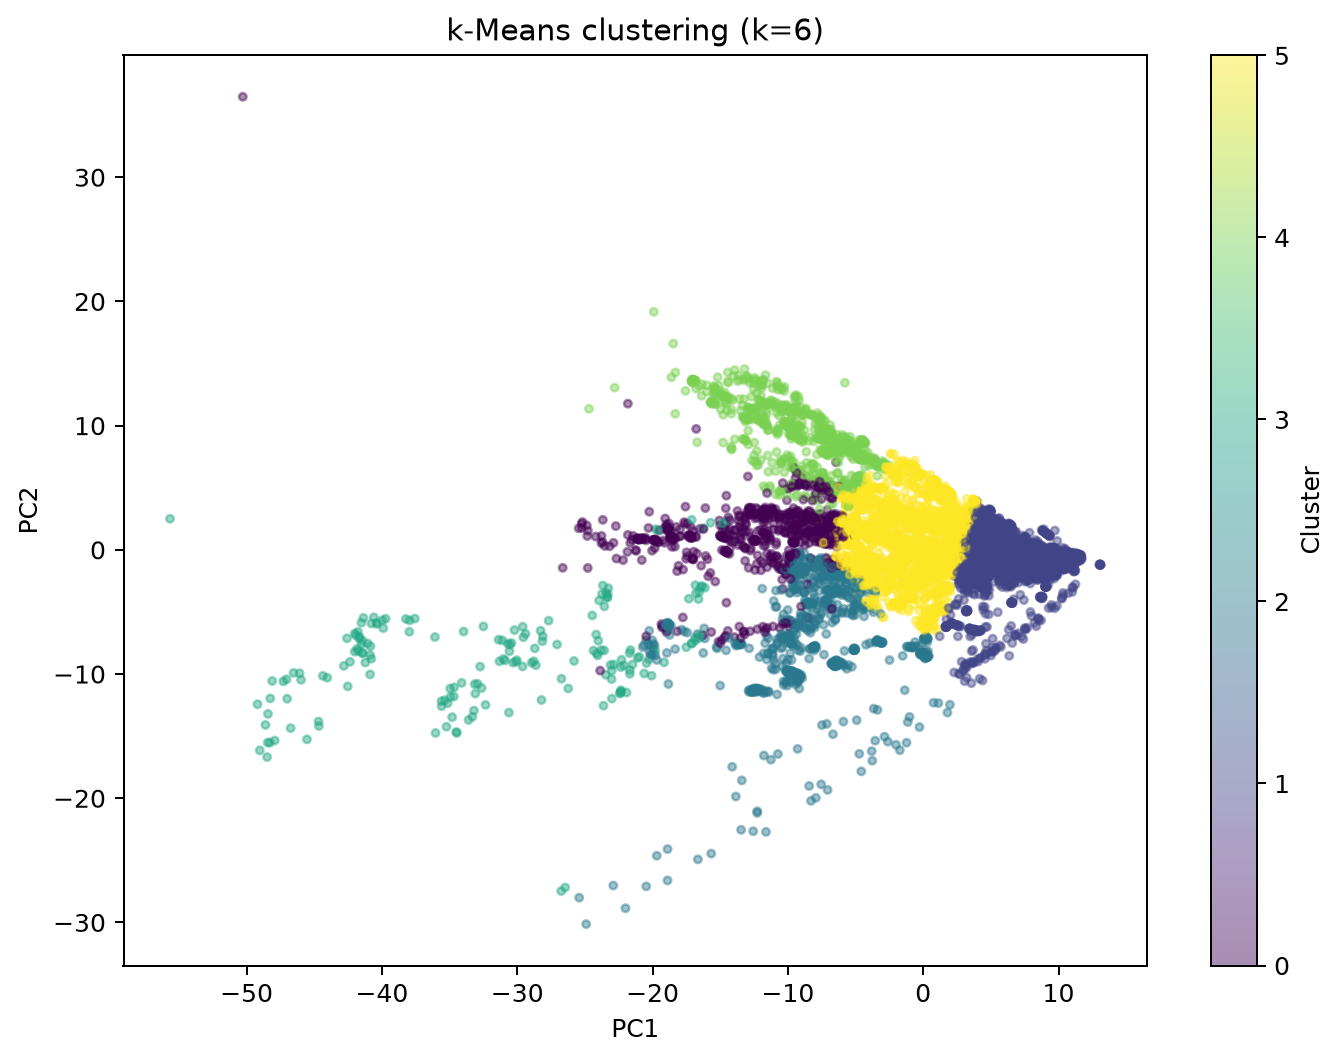
\includegraphics[width=\linewidth]{15_pca_kmeans_k6.png}
\end{minipage}
\hfill
\begin{minipage}{0.48\textwidth}
\centering
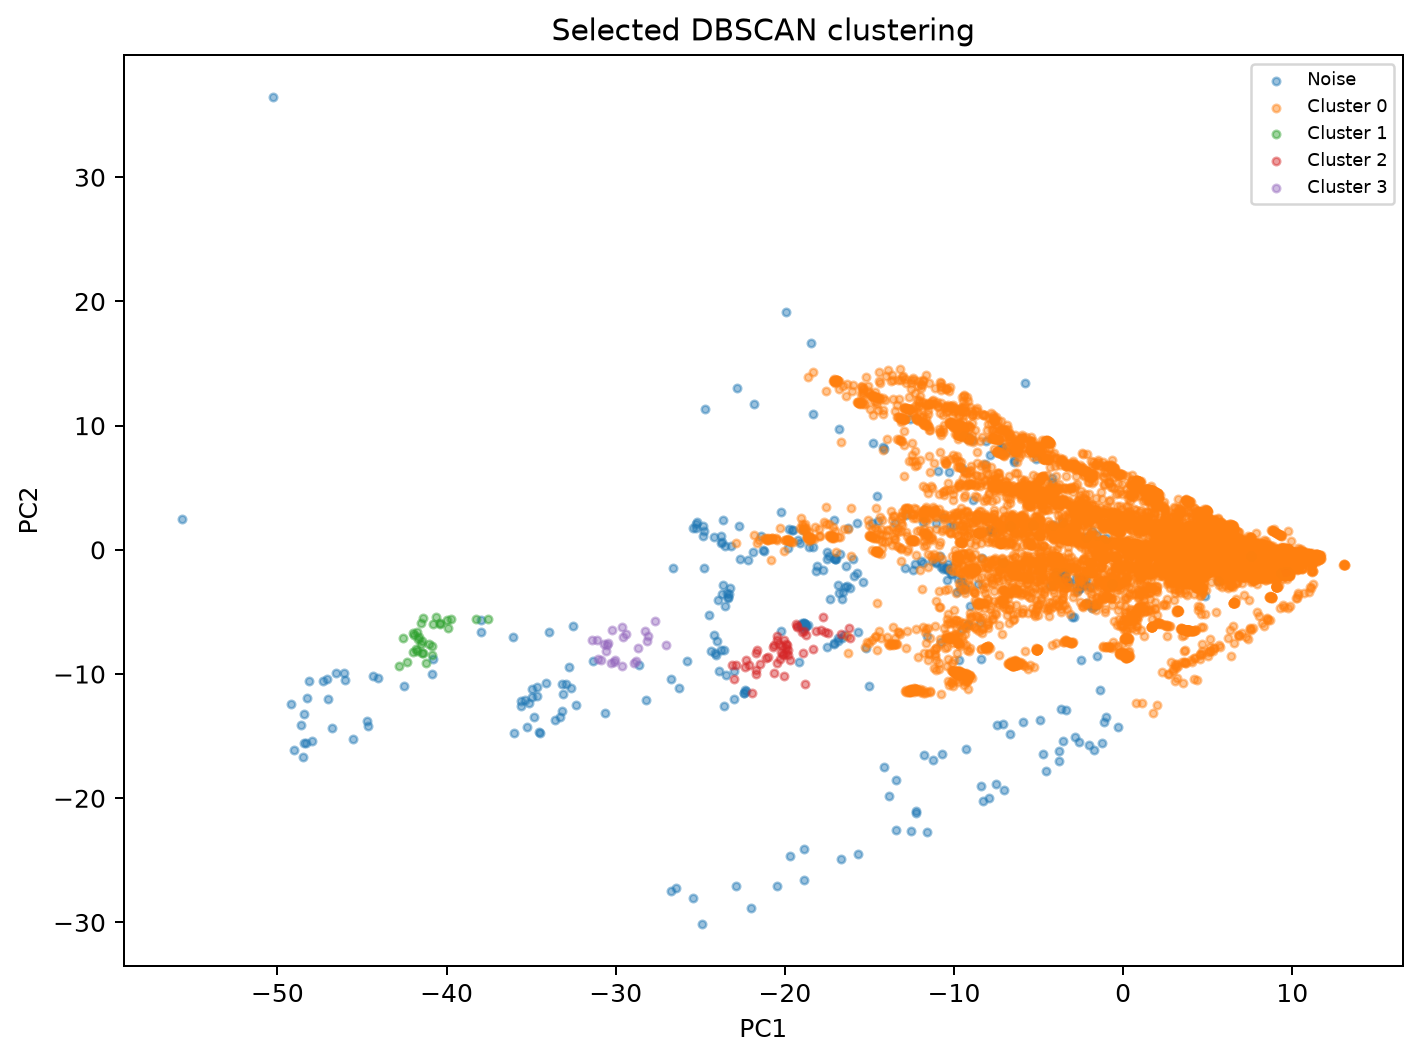
\includegraphics[width=\linewidth]{17_pca_dbscan.png}
\end{minipage}
\caption{PCA projection of the clustering sample colored by the reference k-Means partition ($k=6$, left) and by the selected DBSCAN clustering (right). These plots are exploratory and complement the quantitative summary in Table~\ref{tab:clustering}.}
\label{fig:clustering_algorithms}
\end{figure*}

\subsection{Efficiency Trade-offs}
For temporal classification, MLP achieved the highest observed macro-F1 (0.571) together with the fastest inference among the four learned classifiers (1.223 $\mu$s/sample) and the second-smallest serialized model (0.199~MB); SVM had the smallest serialized model (0.134~MB) but slower inference (2.628 $\mu$s/sample) and lower macro-F1 (0.499). For temporal regression, SVR obtained the lowest RMSE (113.575~ppmv) but the slowest inference among the learned regressors (140.205 $\mu$s/sample, versus 0.843 $\mu$s/sample for XGBoost) and a larger serialized model (2.663~MB versus 0.122~MB for XGBoost); XGBoost obtained an RMSE 5.039~ppmv higher than SVR (118.614 versus 113.575~ppmv) while requiring substantially lower inference time and a smaller serialized model. These trade-offs are visible in Tables~\ref{tab:classification}--\ref{tab:regression}; which model is preferable depends on the relative weight given to predictive accuracy, inference latency, and model size in a given deployment, which this benchmark does not specify.

\section{Discussion}
The FULL experimental run directly demonstrates that mixed-batch and later-batch evaluation answer different questions for this dataset. For classification, macro-F1 falls from 0.996 (best mixed-batch model, XGBoost) to 0.571 (best temporal model, MLP); for regression, RMSE rises from 30.098~ppmv (best mixed-batch model, Random Forest) to 113.575~ppmv (best temporal model, SVR). Both results directly demonstrate a large mixed-batch-versus-later-batch gap for the strongest available model, and both are accompanied by narrow record-level bootstrap confidence intervals (Tables~\ref{tab:classification} and~\ref{tab:regression}), indicating that the gap is stable under resampling of the held-out predictions within each fixed test set. These intervals do not quantify uncertainty across alternative acquisition batches or temporal partitions, so they should not be read as bounding how much the gap would vary under a different later-batch split. What the experiment does not directly demonstrate is the causal source of that gap: the later-batch protocol simultaneously changes the acquisition period, the training-set size (3,633 versus 11,128 training records), and the class and concentration composition of the training data (Table~\ref{tab:data_protocol}; Section~\ref{sec:limitations}). The result is consistent with the sensor-drift motivation of the dataset and with prior cautions about temporal structure in gas-sensor benchmarks \cite{dennler2022}, and it is also consistent with a contribution from the smaller, less diverse later-batch training population; the present design cannot separate these two contributions.

This distinction between direct leakage and temporal confounding is central to interpreting Table~\ref{tab:data_protocol} together with the Results. The direct leakage audit rules out target and metadata leakage and confirms disjoint train/test partitions in both protocols; it does not, and by construction cannot, rule out the indirect batch-associated structure in the sensor features themselves that the later-batch protocol is designed to expose. Near-ceiling mixed-batch performance coexisting with markedly weaker later-batch performance is therefore the expected signature of batch-associated distribution shift under an otherwise clean pipeline, not evidence of an implementation error.

Classification and regression show qualitatively similar mixed-batch-versus-temporal behavior but differ in which model generalizes best: MLP is the strongest later-batch classifier while trailing marginally in the mixed-batch ranking, and SVR is the strongest later-batch regressor while trailing all other learned regressors in the mixed-batch ranking. In both tasks, the model selected exclusively from training cross-validation on the temporal protocol also achieved the highest held-out temporal score in this run; held-out results were not used during model selection. The per-class and per-gas breakdowns (Tables~\ref{tab:per_class} and~\ref{tab:per_gas}) further show that aggregate temporal metrics mask substantial heterogeneity: classification degradation concentrates in specific gases (most severely Toluene), and regression error scales in part with each gas's concentration range.

The clustering results provide a complementary unsupervised view and illustrate that internal cluster validity does not imply semantic alignment with either external label. DBSCAN attains a higher silhouette than the reference k-Means partition, yet both have ARI/NMI values against gas and, especially, against batch that remain low (Table~\ref{tab:clustering}); k-Means shows the comparatively stronger, though still modest, post-hoc alignment with gas identity. Because $k=6$ is fixed to match the known number of gas classes rather than selected by an internal criterion (Fig.~\ref{fig:kmeans_sensitivity}), this alignment should be read as a property of a reference partition, not as evidence that unsupervised clustering discovers gas identity from the sensor features alone. Under the evaluated configuration, the exploratory clustering analysis describes structure in the PCA-reduced feature space rather than establishing a definitive drift mechanism.

Finally, the efficiency results reported above indicate that the model with the strongest held-out temporal score is not always the most computationally efficient one: SVR gives the lowest temporal RMSE but is markedly slower at inference and produces a larger serialized model than XGBoost, whose temporal RMSE is only moderately higher. RQ5 is therefore best answered by reporting predictive performance and efficiency jointly rather than by a single ranking, since the preferred model depends on whether accuracy or inference cost dominates the intended use case.

\section{Limitations}
\label{sec:limitations}
This study uses a public laboratory dataset rather than production industrial sensing data. The available inputs are engineered sensor-response features, not raw sensor time series. The ten batches summarize different acquisition periods and have uneven gas and concentration distributions, so the results should not be generalized automatically to production industrial sensing systems.

The later-batch protocol is a simplified distribution-shift benchmark: it does not implement drift compensation, domain adaptation, recalibration, or continual learning, and it does not isolate sensor drift from other batch-associated factors such as training-set size and class or concentration prevalence. The training population also differs in size between the mixed-batch protocol (a stratified 80\% hold-out of all batches) and the later-batch protocol (batches 1--5 only), so part of the observed degradation may reflect the smaller and less diverse later-batch training set rather than drift alone; this benchmark does not include a matched-training-size or rolling-origin control to separate these effects, and this remains an open direction for future work.

Concentration ranges vary substantially by gas (Table~\ref{tab:per_gas}), so global regression metrics can mask heterogeneous per-gas behavior even where a per-gas breakdown is reported. Hyperparameter search is intentionally bounded to a fixed number of randomized iterations per model and does not guarantee a global optimum. Clustering is exploratory: $k=6$ for the primary k-Means partition is fixed to the known number of gas classes rather than selected by an internal validity criterion, PCA and clustering operate on a bounded sample rather than the full dataset, and ARI/NMI against gas and batch are post-hoc external diagnostics computed after clustering, not optimization targets. Permutation importance is model-dependent and reflects predictive sensitivity of the specific fitted estimator, not a causal or feature-intrinsic property. The reported bootstrap confidence intervals are record-level: they characterize resampling stability of a metric on the fixed held-out predictions of a single protocol instance and do not quantify uncertainty across alternative acquisition batches, alternative temporal partitions, or repeated data collection; a different later-batch split could in principle yield a different gap than the one reported here. Finally, all efficiency measurements (training time, inference time, model size) are specific to the hardware and software versions recorded in the experiment manifest and may not transfer to other environments.

\section{Conclusion}
This paper presents a reproducible benchmark for gas-sensor drift analysis, evaluating gas classification, concentration regression, and exploratory clustering as independently trained tasks under a single auditable pipeline. The modular implementation preserves the original dataset parser, targets, protocols, model families, search spaces, and metrics, while adding a direct leakage audit, bootstrap uncertainty estimates, per-class and per-gas diagnostics, and reproducibility metadata. Under the FULL experimental profile, near-ceiling mixed-batch classification performance (macro-F1 up to 0.996) coexists with substantially weaker later-batch performance (macro-F1 0.571 for the best temporal model), and concentration regression shows an analogous increase in RMSE from 30.098 to 113.575~ppmv for the corresponding best models. The identity of the best-performing model differs between the mixed-batch and later-batch protocols for both tasks, and per-class and per-gas breakdowns show that this degradation is concentrated in specific gases rather than distributed uniformly. These differences are consistent with sensor drift and other batch-associated distribution shifts, and they support the central methodological point of this benchmark: mixed-batch and later-batch evaluation answer different questions and must be reported separately, with explicit uncertainty and per-class detail, when a machine-learning pipeline is applied to a drift-affected sensing dataset.

\section{Data Availability}
The dataset analyzed in this study is publicly available from the UCI Machine Learning Repository as Gas Sensor Array Drift at Different Concentrations, dataset ID 270, DOI: 10.24432/C5MK6M \cite{uci_gas_270}. Raw dataset files are not vendored in the accompanying source-code repository. Instead, the reproducibility pipeline retrieves the canonical UCI archive and verifies its integrity using the archive and per-batch hashes recorded in \texttt{data/data\_manifest.json}.

\section{Code Availability}
The source code, configuration files, tests, and scripts required to reproduce the analyses reported in this study are publicly available at \url{https://github.com/PesquisaDoug/gas-sensor-drift-ml-benchmark}. The results reported in this manuscript correspond to commit \texttt{5ca408022aa5e44fa286116629553cd44d8e2788}, using the FULL experimental profile defined in \texttt{configs/experiment.yaml}. The generated experiment manifest records the source commit, package versions, profile parameters, and execution metadata. Detailed instructions for reproducing the QUICK and FULL workflows are provided in the repository README.

\bibliographystyle{IEEEtran}
\bibliography{references}

\end{document}
